\subsection{JSON-RPC}
JSON-RPC is a \acrfull{rpc} encoded in \acrshort{json}. It is a simple protocol that defines only a few data types and commands. JSON-RPC allows for notifications (data sent to the server that does not require a response) and for multiple asynchronous calls. It uses \acrshort{json} \textit{RFC-4627}\cite{rfc4627} as data format.\\

The first officially released specification was \textit{JSON-RPC 1.0}\cite{json-rpc-1} published in 2005, but the last official specification is \textit{JSON-RPC 2.0}\cite{json-rpc-2} published in 2010 with several improvements.

\subsubsection{JSON}
\acrlong{json} mostly known as \acrshort{json} is a lightweight data-interchange format. It is human readable and easy to write. Also, it is easy for machines to parse and generate. It is based on a subset of the JavaScript Programming Language Standard ECMA-262 3rd Edition - December 1999. \acrshort{json} is a text format that is completely language independent but uses conventions that are familiar to several languages such as \textit{C}, \textit{C++}, \textit{Java}, \textit{JavaScript}, \textit{Perl}, \textit{Python} and many others.\\

\acrshort{json} is built on two structures\cite{jsonSchema}:
\begin{itemize}
    \item A collection of name-value pairs (figure \ref{fig:json_objects}). In various languages, this is realized as an Object, Record, Struct, Dictionary, ...
          \begin{figure}[h]
              \centering
              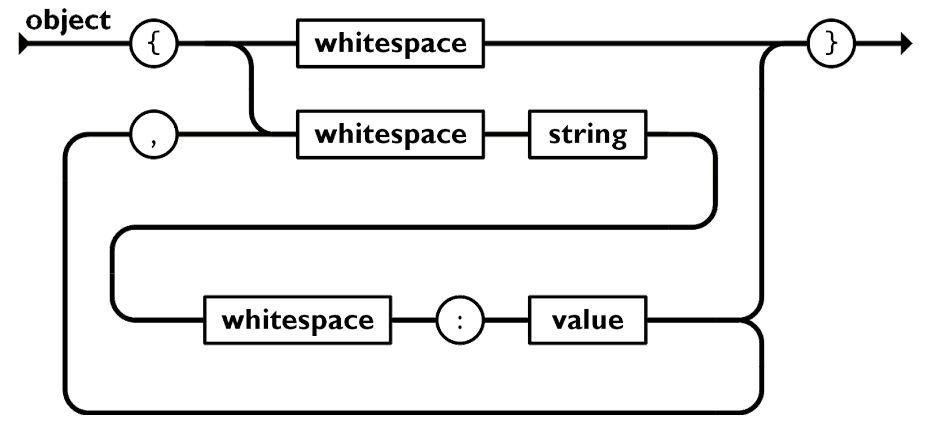
\includegraphics[width=0.6\textwidth]{images/State of the Art/json-rpc/json-objects.png}
              \caption{\acrshort{json} objects schema}
              \label{fig:json_objects}
          \end{figure}
    \item An ordered list of values (figure \ref{fig:json_arrays}). In most languages, this is realized as an Array, Vector, List, ...
          \begin{figure}[h]
              \centering
              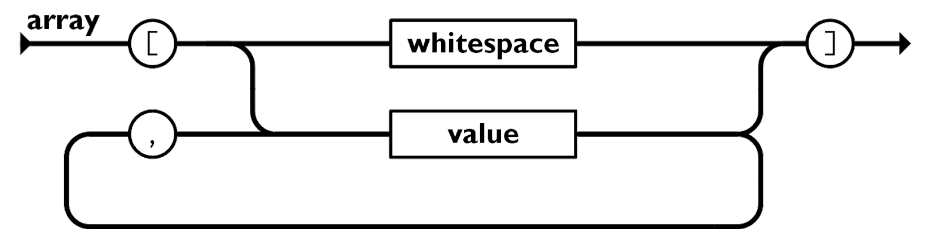
\includegraphics[width=0.6\textwidth]{images/State of the Art/json-rpc/json-arrays.png}
              \caption{\acrshort{json} array schema}
              \label{fig:json_arrays}
          \end{figure}
\end{itemize}

\subsubsection{RPC}
A \acrfull{rpc}\cite{rpc} is when a computer program causes a procedure to execute in a different address space (commonly on another computer), which is coded as if it were a local procedure call. That is, the programmer writes essentially the same code whether the program will run locally or in a remote machine.\\

The transparency is one of the great strengths of \acrshort{rpc}, because the application software does not contain any communication code, it is independent of:
\begin{itemize}
    \item The communication hardware and protocols used
    \item The operative system
    \item The calling sequence needed to use the communication software layer
\end{itemize}

\paragraph{How RPC works}
From the point of view of a remote call, the calling program is known as client, and the subroutine it calls is known as the server\cite{rpcInOS,howRPC}. When the client calls the server, the \acrshort{rpc} system must take care of:
\begin{itemize}
    \item Taking all the parameters which are passed to the subroutine and transferring them to the remote node
    \item Having the subroutine executed on the remote node
    \item Transferring back all the parameters which are returned to the calling routine
\end{itemize}

In the next figure (figure \ref{fig:rpc_schema}) we can see the typical \acrshort{rpc} communication schema.
\begin{figure}[h]
    \centering
    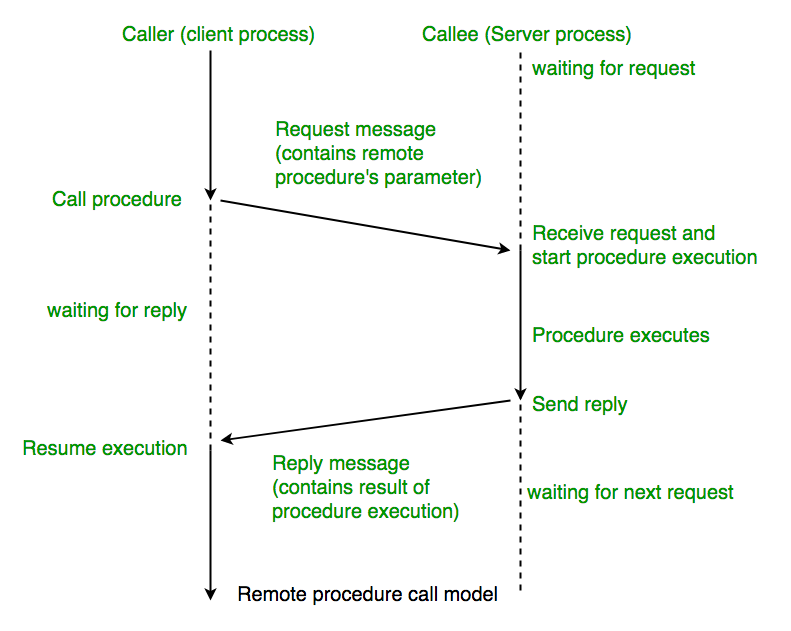
\includegraphics[width=0.7\textwidth]{images/State of the Art/json-rpc/rpc.png}
    \caption{\acrshort{rpc} schema}
    \label{fig:rpc_schema}
\end{figure}
The most common method of doing this is by the use of stub modules (figure \ref{fig:rpc_mechanism}). The client is linked to a client stub module. This is a subroutine which looks like the remote subroutine, but on the inside, it is almost empty. All it does is take the values of the parameters which are passed to it, and put them in a message. This is known as marshalling.\\

The client stub then uses a routine in the \acrshort{rpc} \acrfull{rts} to send the message off and wait for a reply message. When the reply arrives, the stub unmarshals the parameters that were returned in the reply message, putting their values into the variables of the calling program. The client stub then returns to the calling program just like a normal subroutine.\\

The server stub (located in the remote machine) is called by the \acrshort{rpc} \acrshort{rts} when the message arrives from the client. The server stub performs the unmarshall of the parameters passed to the subroutine, calling the subroutine, and marshalling the return parameters.
\begin{figure}[h]
    \centering
    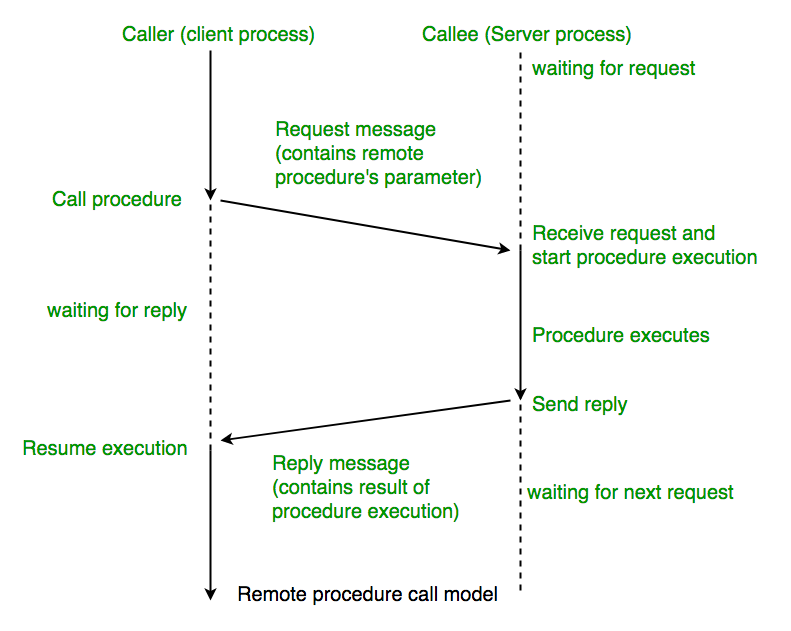
\includegraphics[width=0.7\textwidth]{images/State of the Art/json-rpc/rpc-mecha.png}
    \caption{\acrshort{rpc} mechanism}
    \label{fig:rpc_mechanism}
\end{figure}
All the communication details are handled by the \acrshort{rpc} \acrshort{rts}, so the stubs contain only the code which is specific to the application involved\cite{rpc2}.
\begin{itemize}
    \item In order to produce stub modules, it is need to know
    \item The names of the procedures in the package (set of procedures)
    \item The number of parameters which they take
    \item The data type of each parameter
    \item The direction in which each parameter is transferred
\end{itemize}
\subsubsection{JSON-RPC 1.0}
The general mechanism consists of two peers establishing a data connection\cite{json-rpc-1}. Peers may invoke methods provided by the older peer. To invoke a remote method, a request serialized using \acrshort{json} is sent. The request is a single \acrshort{json} Object with three properties:
\begin{itemize}
    \item \textbf{method}: The name of the invoked method.
    \item \textbf{params}: The params passed as arguments to the method. It is an Array of Objects.
    \item \textbf{id}: The request id. It can be of any type. It is used to match the response with the reply. If it is a notification request, it must be Null.
\end{itemize}
The request must be replied unless it is a notification (does not need a response). The response is also a single Object serialized using \acrshort{json} and has this properties:
\begin{itemize}
    \item \textbf{result}: The Object returned by the invoked method. It is Null in case there was an error.
    \item \textbf{error}: An error Object if there was an error while invoking the method. It is Null if there was no error.
    \item \textbf{id}: The id of the request that was sent.
\end{itemize}
JSON-RPC does not require a certain transport protocol, but \acrshort{tcp}/IP socket streams are encouraged. The request and the response are sent to the peers through byte streams.\\

Also \acrshort{http} can be used as the communication transport. The request must be sent as an \textit{\acrshort{http} POST} with all the serialized Objects. Once the client has received the response, it must reply with another \textit{\acrshort{http} POST}. A non-valid request will result in closing the connection.
\subsubsection{JSON-RPC 2.0}
This specification\cite{json-rpc-2} works almost the same way as the JSON-RPC 1.0 but it has several upgrades.\\

The request Object has the following properties:
\begin{itemize}
    \item \textbf{jsonrpc}: The version of the JSON-RPC protocol. It must be exactly "2.0".
    \item \textbf{method}: A String containing the name of the method.
    \item \textbf{params}: A Structured value (Object or Array) with the parameter values passed as arguments to the method.
    \item \textbf{id}: It is a String, Number or \textit{Null} identifier. If it is not included, it is assumed to be a notification. Normally it should not be \textit{Null} because this specification uses a value of \textit{Null} for responses with unknown id. Also, JSON-RPC 1.0 uses \textit{Null} for notifications, and it causes confusion in handling.
\end{itemize}
Similarly, the response from the server is expressed as a single \acrshort{json} Object with the following properties:
\begin{itemize}
    \item \textbf{jsonrpc}: As in the request, it must exactly be "2.0"
    \item \textbf{result}: It is required on success, but must not exist if there was an error.
    \item \textbf{error}: It is required on error, but must not exist if there was no error. It must be an Object with the following properties:
          \begin{itemize}
              \item \textbf{code}: A Number that indicates the error type occurred.
              \item \textbf{message}: The provided short description of the error.
              \item \textbf{data}: A Primitive (String, Number, Boolean or Null) or Structured (Object or Array) with additional information about the error. This may be omitted and it is defined by the server. The error codes are nearly the same as those suggested for XML-RPC\cite{rpc-err}.
          \end{itemize}
    \item \textbf{id}: This property must be the same as the value of the requested Object. If there was an error, it must be \textit{Null}.
\end{itemize}
To send several requests at the same time, the client may send an Array with all the request objects. It is called batch. The response from the server should be another Array containing the response objects after all the requests have been processed. The server may process the batch as a set of concurrent tasks. Also, the response objects may be returned in any order within the Array. Thanks to the id server and client will match the context between requests and responses.